\documentclass	[11pt, a4paper, openany]{book}
\usepackage[utf8]{inputenc}
\usepackage[francais]{babel}
\usepackage[T1]{fontenc}
\usepackage{amsmath}
\usepackage{amsfonts}
\usepackage{amssymb}
\usepackage{lmodern}
%\usepackage{mathpazo}
%\usepackage[scaled=0.95]{helvet}
%\usepackage{courier}
\usepackage{amsthm}

\usepackage{graphicx} % ajout image
\usepackage[tt]{titlepic}%Centre le titre

\usepackage{shorttoc} %Permet d'avoir de petites tables des matières


\usepackage{shapepar} %texte en keur
\usepackage{siunitx} %S.I.

\usepackage{graphicx}
\usepackage{caption} %Permet d'ajouter des légendes en images sans les mettre en float + ds la marge
\usepackage{delarray} % Belles matrices

\usepackage{fancyhdr} %Permet de modifier l'entête & footer
\usepackage{bbding} % Note marge
\usepackage{todonotes}
\usepackage{wrapfig}

\pagestyle{headings} % Titre du ch et numéro page dans l'entete
\usepackage{fullpage} %Utilise toute la page

\usepackage{adjustbox}% empeche les box de sortir de la page


\newcommand{\prop}[1]{\adjustbox{minipage=\linewidth-2\fboxsep-2\fboxrule,fbox}{\begin{center}
#1\end{center}}}

\newcommand{\cst}{\text{cst}}
\newcommand{\E}{\vec E}
\newcommand{\F}{\vec F}

\newcommand{\corollaire}[1]{\ \\\begin{tabular}{|c}
\begin{minipage}{\textwidth}
  \textsc{Corollaire : } \textit{#1}
\end{minipage}
\end{tabular}}

\newcommand{\questpm}[3]{#1. \textbf{#3} (p.#2)}
\newcommand{\exerc}[2]{\textbf{\Large Exercice #1\normalsize \\#2}}
\newcommand{\dif}{\mathrm{d}}
\newcommand{\comment}[1]{}
\newcommand{\rot}{\text{rot}\,}
\newcommand{\divv}{\text{div}\,}
\newcommand{\phas}[1]{\underline{#1}}
\newcommand{\RE}{\text{Re}}
\DeclareMathOperator{\arccot}{arccot}
\newcommand{\com}[1]{}

%\newcommand{\oiint}{\int\!\!\!\!\!\:\!\!\!\;\!\!\subset\!\!\supset\!\!\!\:\!\!\!\!\!\int}
\newcommand{\oiint}{\int\!\!\!\!\!\!\! \:\!\subset\!\!\supset\!\!\!\!\!\!\!\int}


\newcommand{\danger}{{\huge\fontencoding{U}\fontfamily{futs}\selectfont\char 66\relax}\ }
\begin{document}
\renewcommand{\proofname}{Démonstration}
\frontmatter
%\mainmatter
\begin{titlepage}
\begin{center}	
	
	\newcommand{\HRule}{\rule{\linewidth}{0.5mm}}   			%Titre en gros
	
\includegraphics[scale=0.11]{logo.jpg}~\\[1cm]				%Logo

	\textsc{\LARGE Université Libre de Bruxelles}\\[1.5cm]
	\textsc{\Large Synthèse}\\[0.5cm]

	\HRule \\[0.4cm]
	{ \huge \bfseries Électronique appliquée \\ \ \\ ELEC-H-301 \\[0.4cm] }


	\HRule \\[1.5cm]
		\begin{minipage}{0.4\textwidth}
		\begin{flushleft} \large
		
		\emph{Auteur:}\\
			Nicolas \textsc{Englebert}\\
			\end{flushleft}
			\end{minipage}
			\begin{minipage}{0.4\textwidth}
			\begin{flushright} \large
			\emph{} \\		
			\textsc{}
			\end{flushright}
		\end{minipage}

	\vfill

% Bottom of the page
{\large \today}

\end{center}
\end{titlepage}
\tableofcontents



\mainmatter
\part{Rappels d'électricité}
\chapter{Introduction générale}
\section{L'électronique, c'est quoi ?}
Les slides sont assez informatifs, l'essentiel est repris ci-dessous :\\

\prop{\begin{itemize}
\item L'électronique est la principale technologie pour traiter et
transmettre l'information.
\item Cette information est codée dans un signal électrique
\item Faire de l'électronique, c'est notamment choisir et assembler
des composants
\end{itemize}}


\section{Une vision plus large}
\subsection{Comme ingénieur, votre job est de "contrôler" les choses}
Le \textit{contrôle de processus} est \textbf{la} situation de base
de l'ingénieur. L'électronique est ainsi au cœur des boucles de 
contrôles.

\subsection{Système embarqué}
On appelle \textit{système embarqué} tout objet utilisant de l'
électronique, que ce soit pour une fonction précise, pour de l'
électronique "enfouie" pour doper une fonction de base ou encore
pour satisfaire des contraintes spécifiques.\\

Ajoutons un petit mot sur l'\textit{intelligence}. Celle-ci désigne
une capacité de calcul, c'est à dire l'électronique et donc comme
nous venons de le voir les systèmes embarqués.


\section{Un peu plus d'électronique}
Les disciplines de l'électronique se divisent en deux grandes parties:
\begin{enumerate}
\item Signal ou puissance
\item Analogique ou numérique
\end{enumerate}

Ainsi, suivant le \textit{niveau de puissance utilisé} on distinguera
l'électronique de \textbf{signal} dont le but est de traiter l'information et
ce avec une faible puissance ($mW$ à $W$). C'est l'objet de ce cours. L'électronique de \textbf{puissance} dont le but est de mettre en forme
une puissance électrique ne sera - hélas - pas vu ici. Notons que l'\textit{électronique analogique} travaille par correspondance directe alors que l'\textit{électronique numérique} passe par un codage intermédiaire sous forme binaire.

\newpage


\chapter{Vademecum d'électricité}
\section{Notions fondamentales}
\subsection{Schémas}
Tout schéma possède un sens de lecture, de l'entrée vers la sortie. La \textit{charge}
est le composant connecté en aval d'un montage. Lorsque celle-ci est retirée
le montage fonctionne à vide. La \textit{source} est exactement l'opposé,
c'est à dire le composant connecté en amont d'un montage.

\subsection{Les éléments : dipôles et quadripôles}
\begin{wrapfigure}[4]{r}{3cm}
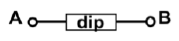
\includegraphics[scale=0.5]{img/image1.png}
\captionof{figure}{Dipôle}
\end{wrapfigure}
Tout élément possède un certain nombre de \textit{bornes} (caractérisée par un potentiel électrique et une valeur de courant\footnote{Lorsque $I$ est identique aux deux bornes, on peut les associer et parler de \textbf{port} ou \textbf{accès}. Le dipôle est par définition un accès.}) qui servent à établir des connexions, un dipôle est simplement un élément en possédant deux.

\subsubsection{Nœud, branche et maille}
\begin{wrapfigure}[9]{l}{6cm}
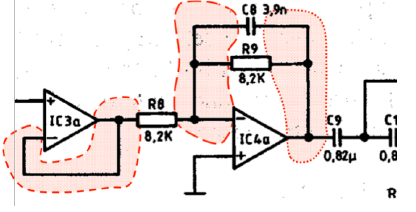
\includegraphics[scale=0.5]{img/image2.png}
\captionof{figure}{Nœud}
\end{wrapfigure}
On connecte les éléments par des bornes : lorsqu'on connecte plusieurs éléments ensemble on forme un noeud, qui est par définition équipotentiel.\\
\textbf{Attention !} Le noeuds couvre l'ensemble de la connexion et pas seulement le point de contact des fils.\\

Tout dipole ou assemblage de dipole en série constitue une \textbf{branche} est l'ensemble de ces branches constituant un parcours fermé constitue une \textbf{maille}.

\subsubsection{Composants en série/en parallèle}
Les deux règles à retenir sont :
\begin{enumerate}
\item Deux composants sont connectés en série s'ils sont parcourus par le même
courant.
\item Deux composants sont connectés en parallèle s'ils sont soumis à la même
différence de potentiel.
\end{enumerate}

\subsection{Courant}
Le \textbf{courant} est un déplacement d'ensemble de charges électriques dans un conducteur.\\
Notons qu'un courant est généralement constitué d'électrons mais que ce-dernier peut également être constitué d'électrolytes ou de semi-conducteurs.

\subsubsection{Intensité = valeur du courant électrique}
L'\textbf{intensité} est le débit de charge électrique :
\begin{equation}
i(t) = \frac{dq(t)}{dt}
\end{equation}

\subsubsection{Mesure du courant électrique}
Il faut insérer un ampèremètre \textbf{en série} avec le fil dans lequel on désire mesurer le courant.

\subsubsection{Représentation du courant : sens conventionnel}
\begin{wrapfigure}[5]{l}{3.5cm}
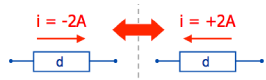
\includegraphics[scale=0.5]{img/image3.png}
\captionof{figure}{Inversion du sens}
\end{wrapfigure}
Il s'agit d'une flèche qui pointe dans la direction de charge qui seraient positives : il s'agit du sens de courant conventionnel qui est toujours représenté dans les schéma.\\
Si le courant était négatif, on peut le rendre positif en inversant le sens de la flèche.

\subsubsection{Circulation du courant en boucle fermée}
"Un chemin de retour" doit toujours exister. Branche interrompue : courant nul.

\subsection{Tension(s)}
\subsubsection{La tension : un terme ambigu}
C'est un terme ambigu car il peut être trois chose distinctes : la force électromotrice, le potentiel d'un noeud ou la d.d.p.

\subsubsection{DDP et potentiel}
\subsubsection{Différence de potentiel}
C'est ce qui se mesure en pratique (à l'aide d'un multimètre, sur un dipôle), il s'agit de la différence de potentiel entre deux bornes.

\subsubsection{Potentiel électrique (première approche)}
C'est une notion purement théorique qui se résume à dire que le potentiel électrique en un point est l'énergie à dépenser pour amener une charge unitaire depuis un point ou le potentiel est nul (à l'infini).

\subsubsection{Convention et signes}
\subsubsection{Convention concernant le sens de la différence de potentiel}
La ddp étant une soustraction, il faut définir le sens de celle ci.
Lorsque la flèche va de $B$ vers $A$ (convention) :
\begin{equation}
V = V_A - V_B
\end{equation}
Ceci découle de cette opération "soustraction", la pointe de la flèche pointera vers le potentiel le plus haut.

\subsubsection{Interprétation des notions de potentiel et de masse}
\subsubsection{Potentiel et masse = notion théorique}
Plus utile que le potentiel, on utilise la masse:\\
\prop{La masse est le noeud dont le potentiel, par convention, est nul : $V_{masse} = 0V$}\ \\

C'est un choix arbitraire, une convention qui servira de référence.
Si on connait toutes les ddp, il faut un "repère" sans quoi on ne pourra jamais connaître les potentiels des noeuds (qui est "défini à une constante près").

\subsubsection{Présence/absence de masse}
On n'a pas besoin de masse pour résoudre un circuit sur papier.\\
\prop{Si l'on ne s'intéresse qu'aux ddps, il n'est pas nécessaire de définir une masse}\ \\

\subsubsection{Potentiel représenté comme une ddp}
\prop{La ddp entre un noeud A quelconque et la masse est numériquement égale au potentiel de ce noeud A}\ \\

\subsubsection{Tension différentielle}
Souvent, en présence de masse, on calcule la ddp par rapport avec celle-ci. Si la masse n'est pas présente on parlera de \textbf{tension différentielle} pour bien différencier les deux.

\subsubsection{Terre = protection}
\begin{wrapfigure}[5]{r}{2.5cm}
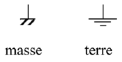
\includegraphics[scale=0.5]{img/image4.png}
\captionof{figure}{Symboles}
\end{wrapfigure}
Il ne faut pas confondre les deux, la terre est une notion pratique relative à la sécurité des personnes et des équipements.

\subsection{Puissane instantanée, conventions et passivité}
\subsubsection{Dipôles actifs et passif - définition intuitive.}
\begin{itemize}
\item[Passif] : Ne peut qu'absorber l'énergie (résistance, condensateur, ...)
\item[Actif] : Injecte de l'énergie dans le circuit (source de tension, pile, ...)
\end{itemize}

\subsubsection{Puissance instantanée sur un dipôle}
La puissance électrique est l'énergie fournie ou reçu par unité de temps par un dipôle
\begin{equation}
p(t) = v(t).i(t)
\end{equation}

\subsection{Conventions récepteurs et générateur}
Dans tout dipôle passif, les flèches courant et tension doivent être de sens opposés : \textbf{convention récepteur}.\\
\begin{wrapfigure}[8]{r}{3cm}
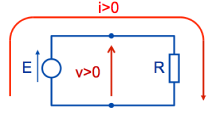
\includegraphics[scale=0.5]{img/image5.png}
\captionof{figure}{Conv. générateur}
\end{wrapfigure} Dans cette convention, la formule $p(t)$ donne la puissance instantanée absorbée par ce dipôle.

Dans la source par contre, ces deux flèches doivent être dans le même sens. La formule de puissance donnera dans ce cas la puissance instantanée fournie grâce à la \textbf{convention générateur}.Le rôle de la source est de "relever" le potentiel.

\subsection{Critère de passivité}
\begin{equation}
w(t) = \int_0^\infty p(t)dt \geq 0
\end{equation}
Un dipôle passif ne peut pas délivrer ce qu'il n'a pas reçu, cela ne peut donc pas être négatif. Si c'est le cas, le dispositif sera \textit{actif}.
 


\newpage
\section{Comportement externe : loi et caractéristique d'un dipôle}
\subsection{Dipôle}
\subsubsection{Etat électrique d'un dipôle}
Il s'agit du couple $(I,V)$ de valeurs électriques mesurables sur un dipôle à l'instant $t$.

\subsubsection{Comportement électrique du dipôle}
Les valeurs que prennent $I$ et $V$.

\subsubsection{Loi du dipôle}
C'est la formule exprimant mathématiquement le comportement.
\begin{itemize}
\item[Source de tension idéale] : $V = E$ : impose une ddp et ce peu importe le courant qui la traverse (ne modifie par le courant).
\item[Source de courant idéale] : $I = J$ : impose un courant et ce peu impporte la tension (ne modifie pas la tension).
\end{itemize}

\subsubsection{Caractéristique}
La \textbf{caractéristique} est la représentation graphique du \textit{comportement électrique} du dipôle.\footnote{La caractéristique n'apporte aucune info supplémentaire par rapport à la loi.}

\setcounter{section}{2}
\subsection{Charges idéales : trois effets physiques}
\setcounter{subsection}{1}
\subsubsection{Inductance}
La loi de base est que $\phi \propto I$ impliquant :
\begin{equation}
\phi (t) = LI
\end{equation}
Comme $v(t) = \frac{d\phi}{dt}$ on peut dire que $v(t) = L\frac{di}{dt}$ et $e(t) = -\frac{d\phi}{dt}$ qui est une autre manière d'exprimer la loi de Lenz. On utilisera :
\begin{itemize}
\item loi de l'inductance : convention récepteur
\item loi de Lenz : convention générateur
\end{itemize}

\begin{center}
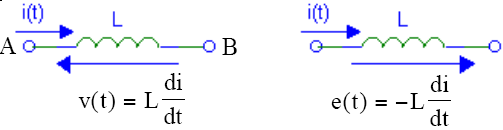
\includegraphics[scale=0.5]{img/image10.png}
\captionof{figure}{Inductance/Lenz}
\end{center}

La loi courant-tension décrite ci-dessus implique :
\begin{itemize}
\item si la ddp est \textbf{constante}, le courant croît \textbf{linéairement}
\item si le courant est \textbf{constant}, la ddp est \textbf{nulle}.
\end{itemize}


\subsubsection{Lois "court terme" et "long terme"}
Dans une self, le courant ne peut pas varier instantanément sinon la ddp serait infinie. Il s'agit de la loi à court terme.\\
Cependant, après un temps infini la ddp doit forcément être nulle sans quoi $I = - \infty$ ce qui est impossible. Il s'agit de la loi à long terme.

\subsubsection{Interprétation physique}
Lorsque 'lon essaye de faire varier le courant dans une self, celle-ci développe une fem qui contre cette variation. La self oppose donc une certaine \textit{inertie} à la variation du courant qui la traverse.\\

Histoire de ne pas l'oublier (et de mettre en avant cet "effet mémoire"), voici la loi courant tension de la self:
\begin{equation}
i(t) = i(0) + \frac{1}{L}\int_0^t v(t) dt
\end{equation}


\subsection{Capacité}
La loi de base à retenir est que $Q \propto V$.
\begin{equation}
i(t) = C \frac{dv(t)}{dt}
\end{equation}
où $v$ est la ddp. On dira que
\begin{itemize}
\item la capa se \textbf{charge} quand la ddp (ou |Q|) \textbf{augmente}
\item la capa se \textbf{décharge} quand la ddp (ou |Q|) \textbf{diminue}
\end{itemize}


\subsubsection{Interprétation physique}
A cause de la dérivée dans cette expression on remarque, à l'inverse de $R$\footnote{Où courant implique tension}, que c'est la \textit{variation de la ddp} qui implique l'existence d'un courant et inversement.\\
Une capacité n'a pas de caractéristique dans le plan $(I,V)$ car le temps y intervient. Retenons que
\begin{enumerate}
\item si le courant est constant, la ddp croit linéairement
\item si la ddp est constante, le courant est nul.
\end{enumerate}

\subsubsection{Lois "court terme" et "long terme"}
On constante que la $ddp$ ne varie pas instantanément sinon $i(t) = \infty$ ce qui est impossible.\\
Après un temps infini, le courant doit forcément être nul sinon la ddp atteindrait une valeur négative infinie ce qui est également impossible.

\subsubsection{Autre interprétation physique}
Pour faire varier la charge, il faut injecter ou retirer des charges à la capacité, ce qui prends un certain temps (pas instantané): il faut qu'un courant circule : on dit que la capacité s'\textbf{oppose/présente une inertie} aux variations de tension

\subsubsection{Charge initiale}
La loi de base exprimée en tension et en courant est 
\begin{equation}
v(t) = \frac{1}{C} \int_{-\infty}^t i(t) dt
\end{equation}
Ou encore, plus pratiquement (ne pas oublier $v(0)$ qui traduit un "effet de mémoire" :
\begin{equation}
v(t) = v(0) + \frac{1}{C} \int_0^t i(t) dt
\end{equation}


\subsection{Court-circuit et circuit ouvert}
\subsubsection{Court-circuit}
Il s'agit d'un dipôle imposant une ddp nulle, quelque soit la valeur du courant qui le traverse : $V = 0$.\\ On réalise un court circuit en mettant deux noeuds au même potentiel.
\textbf{Attention !} Ddp nulle n'implique pas que le courant l'est également !

\subsubsection{Circuit ouvert}
Un \textbf{circuit ouvert} est par définition un dipôle traversé par un courant nul, quelque soit la ddp à ses bornes : $I =0$.\\
\textbf{Attention !} Encore une fois, la ddp aux bornes d'un circuit ouvert est à priori \textbf{non} nulle !




\newpage
\section{Circuits équivalents et théorèmes de Thévenin/Norton}
\subsection{Théorèmes de Thévenin/Norton}
\subsubsection{Équivalence de deux circuits}
\prop{Deux circuits sont équivalents (au sens de Thévenin) s'ils ont la même caractéristique}\ \\

Comme la caractéristique traduit le comportement aux bornes du circuit, cela revient à dire que :\\
\prop{Deux circuits sont équivalents s'ils possèdent le même comportement électrique (vu du circuit extérieur)}\ \\

En régime sinusoïdal, deux dipôles seront équivalent s'ils ont la même impédance.


\subsubsection{Théorème et équivalent de Thévenin}
Le \textbf{théorème de Thévenin} s'énonce :\\

\prop{Tout circuit linéaire et permanent est équivalent à une source de tension unique $V_{th}$ en série avec une impédance $Z_{th}$.}
\begin{center}
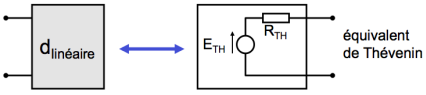
\includegraphics[scale=0.7]{img/image21.png}
\captionof{figure}{Illustration du théorème de Thévenin}
\end{center}
Notons que $V_{th}$ est la tension à vide (ou fem à vide) entre les bornes du réseau (ici $d$ lorsque celui-ci est déconnecté de tout autre réseau. 
$Z_{th}$ est l'impédance, vue des bornes du réseau.


\subsubsection{Théorème et équivalent de Norton}
Le \textbf{théorème de Norton} est une variante du th. de Thévenin, utilisant cette fois une source de courant :\\
\prop{Tout réseau linéaire et permanent est équivalent à une source de \textit{courant} unique $I_N$ en \textit{parallèle} avec une impédance $Z_N$.}
\begin{center}
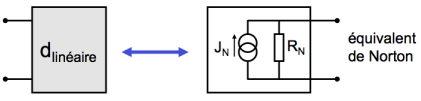
\includegraphics[scale=0.7]{img/image22.png}
\captionof{figure}{Illustration du théorème de Norton}
\end{center}


Une multitude d'exemples d'applications sont disponibles dans les slides (24-31)\\
Les démonstrations de ces théorèmes sont à connaître (slide 31 et page 127-128).

\subsection{Impédance d'entrée, impédance de sortie}
\subsubsection{Équivalent de Thévenin d'un dipôle charge : résistance d'entrée}
Supposons qu'un appareil (une charge) doivent recevoir une tension à ses bornes. S'il est linéaire, il lui correspond un équivalent de Thévenin possédant le même comportement électrique.\\

Pour se faire, on définit la \textbf{résistance d'entrée} $R_{in}$ d'un dipôle charge linéaire comme la valeur de la résistance équivalente (au sens de Thévenin) à ce dipôle. Autrement dit :
\begin{itemize}
\item La valeur de la résistance de l'équivalent de Thévenin du dipôle
\item L'inverse de la pente de la caractéristique de ce dipôle
\item La résistance par laquelle on peut remplacer ce dipôle sans modifier le fonctionnement du circuit extérieur
\end{itemize}\ \\
\prop{La résistance d'entrée est avant tout un \textit{nombre} caractérisant le comportement externe du dipôle ([$\Omega$])}\ \\
Ce n'est donc \textbf{PAS} (sauf exception rare) la résistance qui se trouve à l'entrée du circuit !
\subsubsection{Interprétation}
Si un dipôle possède une résistance d'entrée de $500\Omega$ cela signifie simplement que si on lui applique une tension de $10V$ il consommera comme courant $20 mA$.\\

Cette notion permet de remplacer, du point de vue du circuit extérieur, un montage complexe par une résistance fictive unique.

\subsubsection{Équivalent de Thévenin d'un dipôle source : résistance de sortie et fem à vide}
Pour autant que le circuit soit linéaire, il peut être modélisé par un circuit équivalent de Thévenin. Définissons :
\begin{description}
\item[Résistance de sortie] ; Valeur de la résistance de l'équivalent de Thévenin de ce dipôle.
\item[Fem à vide] ; Valeur de la source de tension idéale de l'équivalent de Thévenin de ce dipôle.
\end{description}

\subsubsection{Interprétation}
\begin{wrapfigure}[8]{r}{3cm}
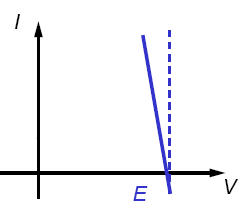
\includegraphics[scale=0.4]{img/image20.png}
\captionof{figure}{Influence de la résistance de sortie}
\end{wrapfigure}
La \textit{fem à vide} est la valeur de la tension visible à la sortie du dipôle lorsque celui-ci ne délivre aucun courant. La tension à la sortie du dipôle valant (dans ce cas $I = 0A$) :
\begin{equation}
V = e_{out} - R_{out}I
\end{equation}
Cette équation permet également de comprendre la \textit{résistance de sortie}. Lorsqu'un courant passe, la résistance de sortie introduit une certaine chute de tension. La tension de sortie est donc plus basse que la fem à vide.\\

\prop{La résistance de sortie traduit la difficulté du dipôle à maintenir sa tension de sortie constante lorsque le courant délivré augmente.}


\setcounter{subsection}{3}
\subsubsection{Équivalent de Thévenin/Norton d'un quadripôle}
\begin{wrapfigure}[8]{l}{4.7cm}
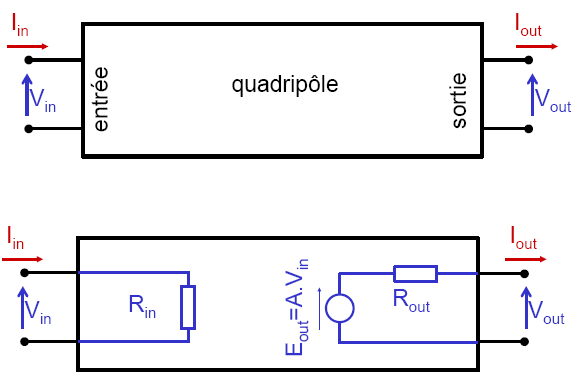
\includegraphics[scale=0.3]{img/image23.png}
\captionof{figure}{Equivalent de Thévenin d'un quadripôle}
\end{wrapfigure}
Il suffit de modéliser l'entrée et la sortie par un équivalent de Thévenin comme précédemment. L'appareil sera caractérisé lors de la connaissances de trois paramètres :
\begin{enumerate}
\item Sa résistance d'entrée $R_{in}$
\item Sa résistance de sortie $R_{out}$
\item Sa fem à vide ($e_{out}$)
\end{enumerate}
Il existe bien entendu cette fois une tension d'entrée, de sortie et même chose pour le courant.


\subsection{Adaptation d'impédance}
\subsubsection{Connecter deux appareils : pas si simple !}
Soit le cas ou on souhaite connecter un apareil en "amont" (source délivrant un signal) à un appareil en "aval" (charge recevant ce signal)\footnote{Chacun de ces appareils sont typiquement des quadripôles.}. Un principe de base est à retenir :\\
\prop{On \textbf{ne} peut \textbf{pas} interconnecter des composants et des montages sans effectuer certaines \textit{vérification}.}\ \\

Il faut :
\begin{enumerate}
\item Vérifier que l'appareil en aval supporte les niveaux de tensions délivrés par l'appareil en amont (risque de dommages)
\item Vérifier l'\textbf{adaptation d'impédance}, c'est-à-dire que les résistance d'entrée et de sortie sont "compatibles".\footnote{On pourrait sinon "bloquer" une grande partie du signal.} Ces critères diffèrent suivant que l'on veut transmettre une tension, un courant ou une puissance.
\end{enumerate}

\subsubsection{Adaptation d'impédance en tension}
Si l'on connecte deux appareil (modélisés par leur équivalent de Thévenin), on modifie la tension présente à l'entrée de l'appareil en aval (gauche) qui ne vaut plus $e$ : formule du diviseur résistif :
\begin{equation}
\left\{\begin{array}{l}
I = \frac{E}{R_{in} + R_{out}}\\
V = R_{in} I
\end{array}\right.
\end{equation}
et donc : 
\begin{equation}
V = \frac{R_{in}}{R_{in} + R_{out}}e
\end{equation}
\begin{wrapfigure}[5]{l}{5.5cm}
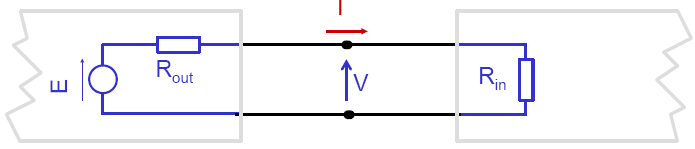
\includegraphics[scale=0.3]{img/image24.png}
\captionof{figure}{Adaptation d'impédance en tension}
\end{wrapfigure}
Le signal de l'appareil en amont est affaibli. Pour éviter toute dégradation, ce "rapport de résistance" doit être proche de l'unité. Le \textbf{critère d'adaptation d'impédance en tension} est donc :\\
\prop{Lorsqu'on désire transmettre un signal de tension, l'impédance de sortie doit être faible devant l'impédance d'entrée.}


\subsubsection{Adaptation d'impédance en courant}
Reprenons le cas de figure précédent si ce n'est que l'appareil en amont se comporte comme une \textbf{source de courant}. La sortie de l'appareil en amont est décrite par un équivalent de \textit{Norton}. Calculons le courant reçu  par l'appareil en aval :
\begin{equation}
\left\{\begin{array}{l}
V = R_{in}\\
V = R_{out}(J-I)
\end{array}\right.
\end{equation}
\begin{wrapfigure}[6]{r}{4.7cm}
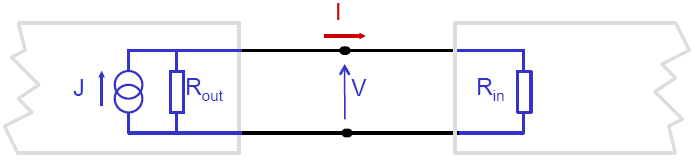
\includegraphics[scale=0.3]{img/image25.png}
\captionof{figure}{Adaptation d'impédance en courant}
\end{wrapfigure}
Le courant dans l'appareil en avant vaut dès lors :

Le signal de l'app
\begin{equation}
I = \frac{R_{out}}{R_{in} + R_{out}}J
\end{equation}
Cette fois, on trouvera une atténuation aussi faible que possible en suivant le \textbf{critère d'adaptation d'impédance en courant} :\\

\prop{Lorsqu'on désire transmettre un signal de courant, l'impédance d'entrée doit être faible devant l'impédance de sortie.}

\subsubsection{Adaptation d'impédance en puissance}
Prenons le cas général ou l'impédance d'entrée $Z_L$ est raccordée à une source de fem vide \underline{$E_S$} et d'impédance interne $Z_S$.\\
Le but est d'optimiser $Z_L$ ($Z_S$ étant supposé fixe) de façon à maximiser la puissance moyenne qu'elle absorbe, en régime sinusoïdal permanent.\\
La démonstration page 144 - 145 du syllabus nous donne le critère tant recherché...\\

\prop{Pour maximiser la puissance transmise de la source à la charge, l'impédance de charge doit être le complexe conjugé de l'impédance de source. \begin{equation}
Z_L = Z^*_S
\end{equation}}


\subsection{Cas particulier des appareils de mesure}
\subsubsection{Connexion d'un appareil de mesure}
Connecter un \textit{voltmètre} ou un \textit{ampèremètre} dans un circuit, cela revient à le modifier ! Analysons ceci grâce aux sections précédentes.\\
\begin{center}
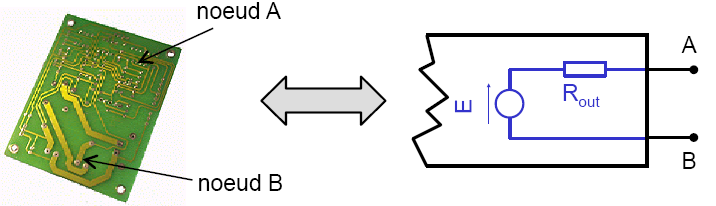
\includegraphics[scale=0.3]{img/image26.png}
\captionof{figure}{Application de l'équivalent de Thévenin}
\end{center}
\textit{Remarque :} Les nœuds choisi pour mesurer une tension (par ex.) ne sont pas forcément des bornes d'entrée/sortie du montage. C'est la encore que l'équivalent de Thévenin va s'appliquer.

\subsubsection{Nœuds à haute et basse impédance}
\subsubsection{Impédance d'un nœud}
\begin{wrapfigure}[6]{r}{3.5cm}
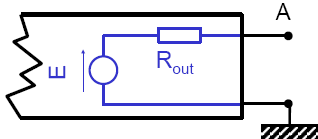
\includegraphics[scale=0.3]{img/image27.png}
\captionof{figure}{Impédance de nœuds}
\end{wrapfigure}
Si l'un des deux nœuds est la masse, le montage est dit \textit{référencé à la masse} (B).\\
L'\textbf{impédance du nœud A} est la résistance de sortie de l'équivalent de Thévenin du montage.\\
On parle de noeud à \textit{haute} ou \textit{basse} impédance suivant la valeur de cette résistance de sortie (typiquement autour de $100 k\Omega$).


\subsubsection{Connexion d'un voltmètre}
\begin{wrapfigure}[6]{l}{4.7cm}
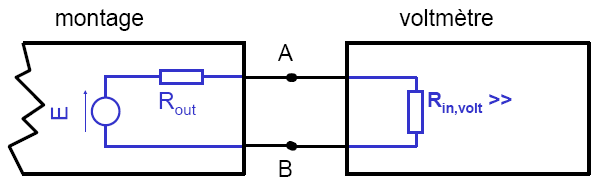
\includegraphics[scale=0.3]{img/image28.png}
\captionof{figure}{Cas du voltmètre}
\end{wrapfigure}
On saura que l'on ne perturbe pas le montage en branchant un voltmètre suivant le critère d'adaptation d 'impédance en tension. Le voltmètre doit avoir \textit{une impédance d'entrée beaucoup plus élevée que l'impédance existant entre les nœuds utilisés pour faire la mesure.}\ \\

\subsubsection{Connexion d'un ampèremètre}
\begin{wrapfigure}[6]{r}{4cm}
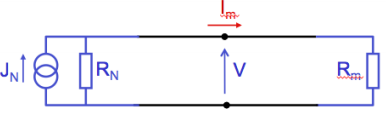
\includegraphics[scale=0.3]{img/image29.png}
\captionof{figure}{Cas de l'ampèremètre}
\end{wrapfigure}
Un  ampèremètre se connecte en \textit{série} pour mesurer un courant, il faut donc obligatoirement interrompre un fil de ce circuit. Il faudra cette fois utiliser un équivalent de Norton. Des résultats précédents, on peut conclure que l'\textit{impédance d'entrée de l'ampèremètre doit être beaucoup plus faible que l'impédance existant entre les nœuds entre lesquels on insère l'ampèremètre}\footnote{Le but est bien d'essayer d'avoir la résistance la plus faible pour se comporter "comme un fil". \textit{Cf. Physique générale - Labo 1}}.





Les composants réactifs ne consomment ou ne génèrent pas de puissance, mais peuvent en stocker momentanément et la restituer ensuite : implique que le \textit{temps} doit être pris en compte.




\newpage
\section{Composants réactifs et outils associés}
\subsection{Analyse temporelle du circuit RC}
\subsubsection{Résolution analytique complète}
Voir syllabus page 201-204.
\begin{center}
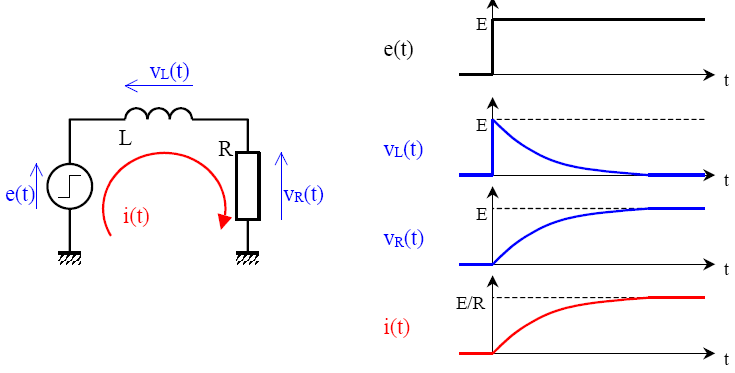
\includegraphics[scale=0.4]{img/image11.png}
\captionof{figure}{Résolution circuit RC}
\end{center}

\subsubsection{Résolution rapide}
\subsubsection{Avant l'échelon (condition initiale)}
\begin{enumerate}
\item Le courant est nul vu la loi à long terme
\item La ddp est constante et supposée nulle (1)
\item La ddp sur la résistance est nulle (2)
\end{enumerate}
\begin{equation}
\left\{\begin{array}{l}
i(t_0^-) = 0\\
v_C(t_0^-) = 0\\
v_R(t_0^-) = 0
\end{array}\right.
\end{equation}

\subsubsection{En t$_0$ (court terme)}
Que ce passe-t-il lorsque l'on applique l'échelon de tension $E$ ?
\begin{enumerate}
\item La ddp de la capa reste nulle (ne peut varier instantanément)
\item En conséquence de (1), toute la tension se reporte sur $v_R$
\item Le courant est donné par Ohm
\end{enumerate}
\begin{equation}
\left\{\begin{array}{l}
v_C(t_0^+) = v_C(t_0^-) = 0\\
v_R(t_0^+) = E\\
i(t_0^+) = E/R
\end{array}\right.
\end{equation}

\subsubsection{En $t = \infty$ (long terme)}
\begin{enumerate}
\item Le courant est nul dans la capacité (loi long terme)
\item En conséquence de (1) la ddp sur la résistance est nulle
\item Toute la tension est reportée sur la capa : $v_C = E$.
\end{enumerate}

\subsubsection{Résolution rapide (2e exemple) : échelon des tension inverse}
En partant de la situation finale du cas précédent, voyons ce qui se passe en appliquant une tension négative d'amplitude E. On suppose que l'instant $t=0$ représente le moment de retour à 0 de la tension $e(t)$.

\subsubsection{Avant l'échelon (conditions initiales)}
\begin{enumerate}
\item Le curant et la ddp sur la résistance sont nuls
\item La ddp sur la capa vaut E (capa chargée)
\end{enumerate}

\subsubsection{En $t_0$ (court terme)}
Juste après l'échelon négatif $-E$
\begin{enumerate}
\item La source de tension prend la valeur nulle ! $e(t_0^+) = 0$
\item La ddp de la capa ne peut pas varier directement : elle vaut encore $+E$
\item En conséquence, la tension de la résistance vaut $-E$
\item Le courant vaut donc $-E/R$
\end{enumerate}

\subsubsection{En $t = \infty$ (long terme)}
\begin{enumerate}
\item Le courant est nul dans la capacité (loi long terme)
\item La tension est nulle dans la résistance à cause de (1)
\item comme $v_R$ et $e(t)$ sont nulles, $v_C$ l'est aussi (capacité complètement déchargée)
\end{enumerate}
\begin{center}
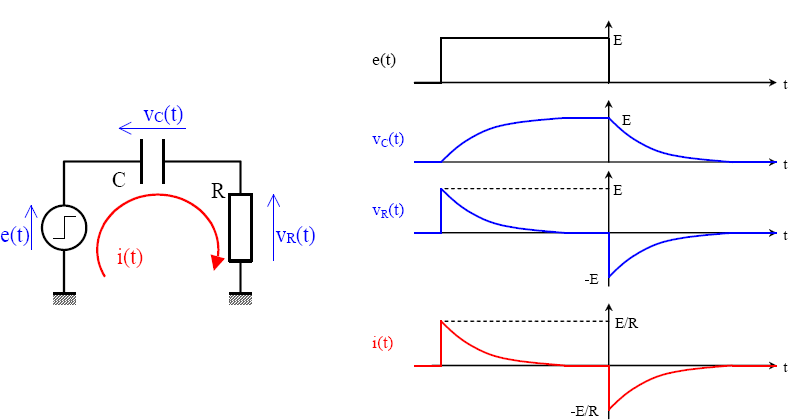
\includegraphics[scale=0.4]{img/image12.png}
\captionof{figure}{Résolution circuit RLC en tension inverse}
\end{center}

\subsubsection{Constante de temps et fréquence de coupure (circuit du 1er ordre)}
La durée de la charge et décharge de la capacité dépend de la constante de charge : $\tau = RC$.
\begin{center}
\begin{tabular}{|c|c|}
\hline 
Temps écoulé depuis l'échelon & Pourcentage de la (dé)charge réalisé \\ 
\hline 
$\tau$ & 63 \\ 
\hline 
$3\tau$ & 95 \\ 
\hline 
$5\tau$ & 99 \\ 
\hline 
\end{tabular} 
\end{center}
On dira également que
\begin{itemize}
\item $v_C(t)$ est un filtre passe-bas de $e(t)$
\item $v_R(t)$ est un filtre passe-haut de $e(t)$
\end{itemize}
La limite entre les fréquences hautes et basses est donnée par la fréquence de coupure définie par
\begin{equation}
f_0 = \frac{1}{2\pi\tau}
\end{equation}
\subsection{Analyse temporelle du circuit RL}
\subsubsection{Résolution analytique complète}
Si l'on attend suffisamment longtemps, par la loi \textit{long terme} $V = 0$ sur la self et $I = cste$ (pas forcément nul).\\
On peut résoudre ce circuit analytiquement (syllabus page 212, slide 54- 57)

\subsubsection{Résolution rapide}
Même raisonnement que pour le circuit RC (page 212 pour le RL)

\subsubsection{Constante de temps et fréquence de coupure}
Les résultats ci-dessus nous apprennent que
\begin{itemize}
\item La tension $v_L(t)$ ne comporte que les hautes fréquences du signal $e(t)$ : filtre passe-haut
\item La tension $v_R(t)$ ne comporte que les basses fréquences
\end{itemize}
 


\subsection{Analyse temporelle du circuit RL (source sinusoïdale)}
Au lieu d'avoir $e(t) = cste$, on a $e(t) = V_m\cos(\omega t + \alpha)$
\begin{equation}
Ri + L\frac{di}{dt} = e(t)
\end{equation}
Il suffit après de résoudre l'équation différentielle comme au cours d'Analyse I.

\subsection{Circuit RLC avec précharge}
La capacité à été préalablement chargée avec une tension $v_0$ et à l'instant $t=0$ on ferme l'interrupteur. L'équation du circuit est donc :
\begin{equation}
v_0 - \frac{1}{C}\int_{t_0}^t i(t)dt = L\frac{di}{dt} + Ri(t)
\end{equation}


\subsection{Fonctions de transfert}
\subsubsection{Plan de Bode}
La fonction de transfert $H(j\omega)$ est le rapport des phraseurs d'entrée et de sortie. C'est l'"opération" réalisée par le circuit. Elle se présente généralement :
\begin{equation}
H(j\omega) = A(\omega)e^{j\phi(\omega)}
\end{equation}
où $A(\omega)$ est l'amplitude et $\phi(\omega)$ la phase\footnote{Attention, $H(j\omega)$ n'est \textbf{pas} un phaseur !}.\\

Les fonctions de transferts sont représentées dans le \textit{plan de Bode} :
\begin{description}
\item[Gain] : Graphique bilogarithmique (log[$A(\omega)$] = f(log($\omega$))
\item[Phase]: Graphique semi-logarithmique ($\phi(\omega)$ = f(log($\omega$))
\end{description}

\subsubsection{Décibels}
C'est une unité adimensionelle pour exprimer un rapport, comme par exemple le rapport de tension ou de courant :
\begin{equation}
X[dB] = 20\log(X)
\end{equation}

Plus utile encore, le rapport de puissances :
\begin{equation}
X(dB] = 10\log(X)
\end{equation}
Son intérêt se trouve dans le fait que les équipement électroniques sont composés de modules successifs, il suffira dès lors d'additionner des décibels de chaque module.



\part{Aspects technologiques}
\setcounter{chapter}{2}
\chapter{Welcome to the real world!}

\section{Signaux analogiques}
\subsection{Perturbations et imperfections}
Un signal analogique n'est pas si idéal que ça, plusieurs formes de perturbations peuvent se manifester comme le bruit, c'est à dire une variation aléatoire du signal autour de sa moyenne mais encore de l'offset, des pics, oscillation, ...\\
L'origine de ses perturbation vient de l'imperfection des composants. On en distingue trois types :
\begin{enumerate}
\item Sources de bruit
\item Dipôles parasites
\item Couplages parasites
\end{enumerate}
Ainsi un bout de fil génèrera un bruit thermique, typique aux métaux.

\subsection{Rapport signal/bruit}
Afin de caractériser ce bruit, on a défini le \textit{signal-to-noise ration} :
\begin{equation}
SNR = 20\log\left(\dfrac{V_{eff}(\text{signal utile + perturbation})}{V_{eff}(\text{perturbations})} \right)
\end{equation}
Celui-ci est exprimé en \textbf{dB} et doit être le plus élevé possible.

\subsection{Bruit}
Le bruit possède deux propriétés : la variation aléatoire du signal et l'origine interne du composant (processus physique fondamental). La conséquence du bruit est le \textit{"plancher" fondamental}. Celui-ci dénote le fait que le bruit ne peut être totalement éliminé et fixe une limite stricte à la précision de l'information.

\subsection{Dipôles parasites}
\textit{Des dipôles parasites sont des phénomènes physiques non désirés mais inévitables}, des effets secondaires qui sont modélisable sous la forme d'un dipôle électrique (comme une résistance accompagnant une self).\\
Les conséquences de ses dipôles parasites se font ressentir dans une limitation de vitesse de réponse (variation d'énergie dans les composants réactifs), des oscillation parasites (résonance du circuit LC ou encore des chutes de tension (résistives ou inductives)


\subsection{Couplages}
Par définition "\textit{Coupage = parasites}". C'est la pollution d'un signal utile par un signal extérieur. A la différence du bruit, son caractère n'est pas forcément aléatoire et son origine est externe au composant.\\
Il existe plusieurs types de couplages :
\begin{description}
\item[Galvanique]; par un conducteur commun
\item[Inductif]; par un champ magnétique (f.e.m. idnuite (Lenz))
\item[Capacitif]; par un champ électrique
\item[Radiatif]; par une onde EM
\end{description}


\subsection{Conclusion}
Du à la complexité du monde réel, il faudra parfois approfondir le modèle pour tenir compte d'effets du deuxième ordre et faire de la \textit{compatibilité électromagnétique}\footnote{Problèmes de câblages, blindages, ...} (CEM).


\section{Résistances}
\subsection{Résistances ordinaires}
\subsubsection{Propriété d'une résistance réelle}
\begin{wrapfigure}[11]{l}{5.9cm}
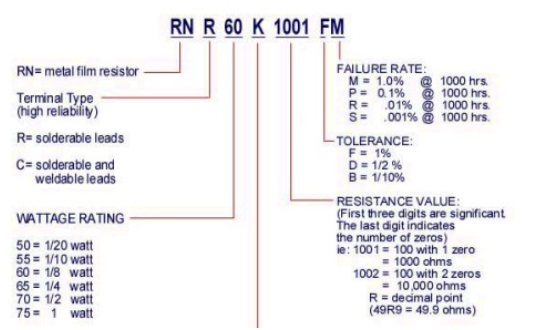
\includegraphics[scale=0.4]{img/image30.png}
\captionof{figure}{Data-sheet d'une résistance}
\end{wrapfigure}
Il existe deux grands procédés de fabrications : les résistances à fil bobiné et les résistance au carbone.\\
Il est important de savoir que la résistance n'a pas pour seule propriété sa valeur ohmique, dictée par la loi d'Ohm $V = RI$. On retiendra ses limites d'utilisations :
\begin{itemize}
\item Limite de puissance
\item Limite de tension
\item Limite de température
\end{itemize}
Au dela de ces limites, il faut également noter des écarts par rapport à la loi idéales, notamment la \textbf{tolérance} (précision sur $R$) et le coefficient de température ($R = f(T)$).

\subsubsection{Valeurs disponibles}
Afin de s'y retrouver, elles sont organisées en séries mais l'important est que l'on peut obtenir quelconque valeur par mise en série et en parallèle. Le marquage de la résistance permet d'obtenir d'avantage d'informations sur celle-ci.

\subsubsection{Utilisation d'une résistance}
Avec une unique résistance, on retrouve les propriétés vue en électricité : conversion courant-tension, limitation du courant,  ... On peut également "découpler" des nœuds (permet que deux nœuds reliés soient à des potentiels différents) mais aussi de fixer le potentiel par défaut d'un nœud avec des résistance de pull-up et de pull-down.


\subsection{Résistances de puissance}
Le but d'une résistance de puissance est de dissiper une certaine puissance en pertes joules.

\subsection{Ajustables et potentiomètres}
\begin{wrapfigure}[9]{r}{3cm}
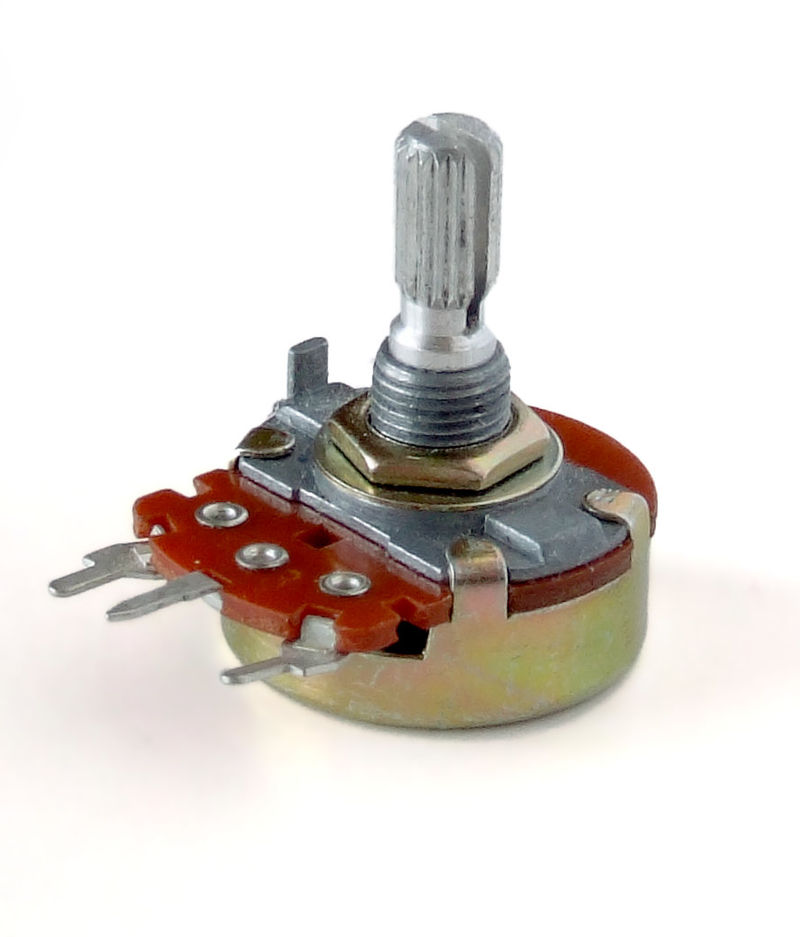
\includegraphics[scale=0.1]{img/image31}
\captionof{figure}{Potentiomètre}
\end{wrapfigure}

Il s'agit de résistances variables, fonction de la position. Elles se composent de trois bornes et suivent une loi de variation. Leur ajustement peut par exemple se faire par tournevis.\\

Le \textit{potentiomètre} (ou \textit{potar}) est un type de résistance variable à trois bornes, dont une est reliée à un curseur se déplaçant sur une piste résistante terminée par les deux autres bornes. Ce système permet de recueillir, entre la borne reliée au curseur et une des deux autres bornes, une tension qui dépend de la position du curseur et de la tension à laquelle est soumise la résistance\footnote{Source : Wikipédia}.

\subsection{Autres types de résistance}
\subsubsection{Thermistance}
\begin{wrapfigure}[6]{l}{3cm}
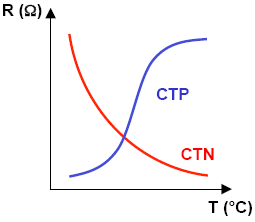
\includegraphics[scale=0.3]{img/image32}
\captionof{figure}{Thermistance}
\end{wrapfigure}
La \textit{thermistance}, un résistance qui dépend de la température, faite en matériau semiconducteur. Son comportement est fortement non linéaire. Il en existe deux types :
\begin{enumerate}
\item CTN - capteur de température de faible précision
\item CTP - pour la protection
\end{enumerate}%\ \\

\subsubsection{Photorésistance}
Celle-ci se base sur le principe $LDR$ - \textit{light dependent resistor}. La résistance est fonction de l'éclairement ; elle est munie d'un capteur. 



\section{Condensateurs}
\subsection{Deux types de condensateurs}
La fonction $Q = CV$ définit la notion de \textit{capacité}qui n'est pas à confondre avec le composant réel : le \textit{condensateur}. Il en existe plus de vingt types différents, mais seulement deux familles : 
\begin{enumerate}
\item Polarisés
\item Non polarisés
\end{enumerate}

\subsection{Condensateurs non polarisés}
\begin{wrapfigure}[6]{r}{3cm}
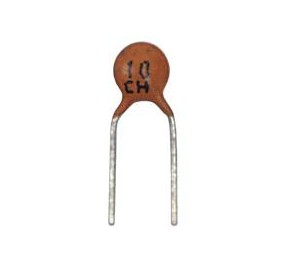
\includegraphics[scale=0.2]{img/image33}
\captionof{figure}{Condensateur céramique}
\end{wrapfigure}
Ceux-ci n'ont pas de "sens" électrique préférable et sont généralement de "faible" valeur (du $pF$ au $\mu F$). Les "classiques" sont les condensateurs céramiques et ceux à films plastiques.\\

On les définit par leur capacité $C$, leur tension de service (50 à 400 $V$) et leur précision (maximum 10\%).

\newpage
\subsection{Condensateurs polarisés}
\begin{wrapfigure}[8]{l}{3cm}
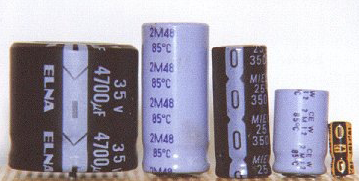
\includegraphics[scale=0.2]{img/image34}
\captionof{figure}{Condensateurs polarisés}
\end{wrapfigure}
Ceux si possèdent un sens électrique (\textbf{risque d'explosion} si monté à l'envers !). Ils supporent une tension DC\footnote{Continue} ainsi qu'une faible composante AC\footnote{Alternative}. Son "sens" d'utilisation se discerne par une "bague".\\

Son principal avantage est de pouvoir stocker une énergie plus importante (coefficient de capacité de $1\mu F$ à quelques $mF$) mais au prix d'une précision médiocre (au mieux 20\%) et d'un encombrement non négligeable. Ceux-ci sont généralement de type électrochimique ($Al$) ou au tantale.


\subsection{Utilisations des condensateurs}
Rappelons que l'impédance d'un condensateur varie en fonction de la fréquence ("infinie" en continu et faible à HF). Il permet de "\textit{séparer}" le continu de l'alternatif. Plusieurs utilisations sont possible :
\begin{description}
\item[Condensateur de liaison]; entre deux étages d'un montage, laisse passer l'alternatif (signal) mais bloque le continu( polarisation)
\item[Condensateur de découplage ]; "court-circuite" un élément de polarisation en HF
\item[Filtrage, réserve énergie, conversion charge-courant, ...]
\end{description}\ \\
Dans les circuits digitaux, on utilise des inductance pour de longues pistes en HF. Ces selfs causent des chutes de tensions inductives (pics\footnote{A cause des commutations}) qui peuvent être absorbées par des condensateurs.\\
On utilisera les condensateurs non-polarisés comme "réserve locale" près des circuits (bon comportement en HF mais peu d'énergie) et préfèrera les polarisés (mauvais comportement HF mais beaucoup d'énergie) à l'entrée de montage pour compenser des variations lentes, mais importantes\footnote{A CLARIFIER}.

\subsection{Autres types de condensateurs}
Il existe également des condensateurs variables mais également des "supercapacités" de l'ordre du farad ! 


\section{Autres composants}
\subsection{Relais}

\textit{Un \textbf{relais} électromagnétique est un organe électrique permettant de dissocier la partie puissance de la partie commande  : Il permet l'ouverture/fermeture d'un circuit électrique par un second circuit complètement isolé (isolation galvanique) et pouvant avoir des propriétés différentes.}\footnote{Source : Wikipédia}\\

\begin{wrapfigure}[8]{r}{2cm}
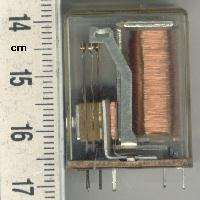
\includegraphics[scale=0.25]{img/image35}
\captionof{figure}{Relais}
\end{wrapfigure}Le principe est donc celui d'un interrupteur commandable électroniquement, basé sur un électroaimant (l'interrupteur mécanique étant trop lent).\\
Son utilisation d'interface entre niveaux de puissances différents permet de commander une grosse puissance au moyen d'une petite (TWSS).


\section{Circuits imprimés}
Un circuit imprimé (PCB - \textit{Printed circuit board}) est un support permettant de relier électriquement un ensemble de composants électroniques. Il ne faut \textbf{pas} le confondre avec un circuit intégré.\\
Ces plaques, recouvertes de substrats isolants sont munies de couches conductrices par gravure chimiques. 


\section{Types de composants}
\subsubsection{Composants classiques >< SMD}
Les composants \textbf{classiques} traversent le substrat et la soudure se fait du côté opposé au composant. Les composants à \textbf{montage de surface} utilisent le SMD (\textit{Surface mount device}), un collage et soudure du même coté du PCB. Cela permet des composants très miniaturisés mais bonne chance pour les réparations.


\subsubsection{Composants discrets >< intégrés}
Les composants \textbf{discrets} ne réalisent qu'une fonction élémentaire unique (R, L, C, diode, transistor, ...) alors que les composants \textbf{intégrés} comportent généralement une "puce" composée de beaucoup de transistors et ayant des fonctions plus ou moins complexes (AOP, microprocesseur, ...).




\part{Électronique analogique}
\setcounter{chapter}{3}
\chapter{L'amplificateur opérationnel}
\setcounter{section}{-1}
\section{Pourquoi amplifier}
L'amplification est omniprésente en électronique analogique. On la réalise avec l'\textit{amplificateur-opérationnel} (composant) bien que le \textit{transistor} soit également fondamentalement un amplificateur. Trois des $6*10^{34}$ raisons d'amplifier sont par exemple : 
\begin{enumerate}
\item Signaux très faibles
\item Réglage de niveau
\item Amplification en amont d'un convertisseur analogique/numérique (CAN)
\end{enumerate}

Dans une  table de mixage analogique signal initial étant relativement faible (venant par exemple d'un micro), les \textit{pré-amplis} servent à augmenter son niveau vis-à-vis des parasites. Ensuite, dans chaque voie, des \textit{amplis} servent à régler le niveau des signaux (pour le mixage).



\section{Ampli-op : propriétés de base}
\subsection{Qu'est ce qu'un ampli-op ?}
\begin{wrapfigure}[5]{r}{2cm}
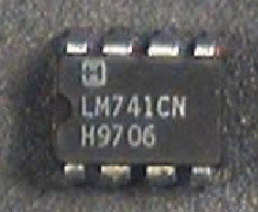
\includegraphics[scale=0.25]{img/image37}
\captionof{figure}{AOP}
\end{wrapfigure}

Un ampli-op se présente le plus classiquement sous forme d'un circuit intégré à huit "pattes". Il s'agit d'un composant à \textbf{deux} bornes d'entrée et \textbf{une} borne de sortie. Conventionnellement, en électronique analogique, le triangle est son symbole.
\begin{center}
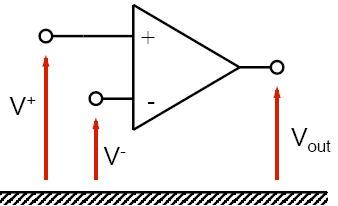
\includegraphics[scale=0.4]{img/image38}
\captionof{figure}{Représentation schématique d'un AOP}
\end{center}
Les deux bornes sont respectivement notée "+" et "-" et correspondent respectivement à l'\textit{entrée inverseuse} et à l'\textit{entrée non-inverseuse}.

\subsubsection{Tension d'entrée et de sortie}
Chacune des \textit{entrées} reçoit un signal de tension mesurée par rapport à la masse : $V^+$ et $V^-$. Même topo pour la tension de sortie $V_{out}$.\\
La fonction d'un AOP est d'amplifier la \textbf{différence} $V_d$ des tensions présentes à ses bornes. Il s'agit de la \textit{tension d'entrée différentielle\footnote{On retrouve la notion de tension différentielle vu au cours \textit{Électricité : ELEC-H-200} signifiant ici qu'aucune des deux bornes n'est la masse.}}

\subsubsection{Loi fondamentale et gain}
Cette fonction d'amplification se traduit mathématiquement par la loi : 
\begin{equation}
V_{out} = A.V_d
\end{equation}
où $A$ est le gain de l'AOP, c'est à dire le facteur\footnote{Sans dimension.} d'amplification de son entrée différentielle et sa sortie.\\
Quelques remarque importantes sont à considérer :
\begin{itemize}
\item Le gain $A$ est toujours très élevé : 30,000 à 100,000 $\rightarrow$ il sera considéré infini.
\item Un tel gain n'a de sens que si le signal d'entrée est très faible : c'est le cas pour $V_d$ ($\ll 1\ mV$).
\item $V_d$ et $V_{out}$ sont de signes quelconques.
\end{itemize}
Le schéma ci-dessous récapitule les concepts précédents et les deux relations à retenir :
\begin{center}
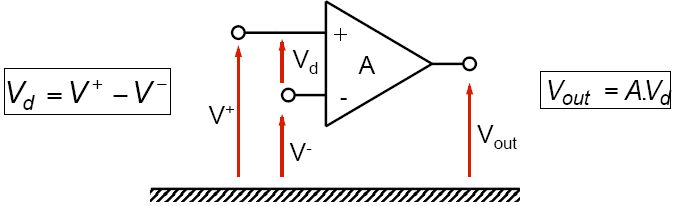
\includegraphics[scale=0.5]{img/image39}
\captionof{figure}{Schéma de synthèse}
\end{center}


\subsubsection{Tensions et bornes d'alimentation}
\begin{wrapfigure}[8]{l}{3cm}
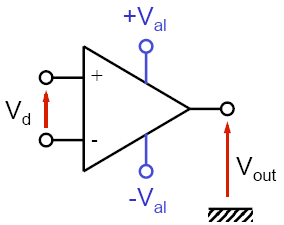
\includegraphics[scale=0.3]{img/image40}
\captionof{figure}{Alimentation}
\end{wrapfigure}
Afin d'amplifier le signal, l'AOP doit être lui même alimenté en énergie : il possède en plus de ses bornes d'entrée et de sortie des bornes d'alimentations $+V_{al}$ et $-V_{al}$. \\

Ces tensions à fournir sont le plus souvent symétriques et valent typiquement +12V/-12V ou +15V/-15V. L'AOP est donc un composé \textit{actif}.\\

Un \textit{quadripôle actif} est défini par le fait qu'un signal de puissance élevée (sortie) est contrôlé par un signal de puissance plus faible (entrée), ce qui est typiquement le cas de notre AOP.\\

\prop{La tension de sortie ne peut pas sortir de la gamme fixée par ces tensions d'alimentations.
\begin{equation}
-V_{al} \leq V_{out} \leq V_{al}
\end{equation}}



\newpage

\subsection{Impédances d'entrée et de sortie}\begin{wrapfigure}[1]{r}{3cm}
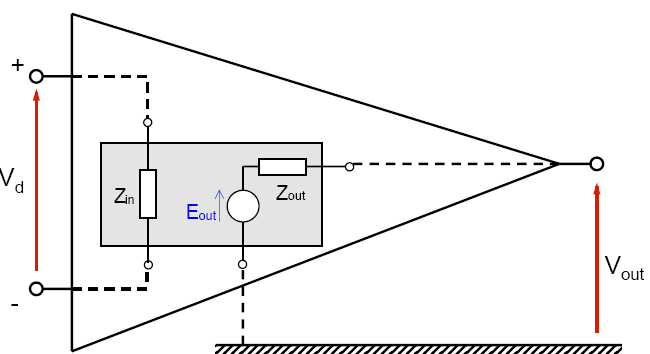
\includegraphics[scale=0.23]{img/image41}
\captionof{figure}{E. Thévenin}
\end{wrapfigure}
\subsubsection{Équivalent de Thévenin}

Pour modéliser l'équivalent de Thévenin, il faut tenir compte de deux particularités de l'AOP :
\begin{enumerate}
\item L'impédance d'entrée $Z_{in}$ est différentielle
\item Au contraire, la source $E_{out}$ est référencée à la masse.
\end{enumerate}


\subsubsection{Valeur des impédances}
L'impédance d'entrée (différentielle) d'un AOP est \textbf{très élevée} ($>\ 10\ M\Omega$). Cela à pour conséquence que le courant signalant entre la borne "+" et "-" est très faible. On considèrera cette impédance comme infinie.\\
L'impédance de sortie est \textbf{très faible} ($\approx 1\ \Omega$). On fera souvent l'approximation que celle-ci est nulle. En résumé : 1. Impédance d'entrée (très) élevée et 2. Impédance de sortie (très) faible.\\
Un AOP convient donc, à priori, pour une \textit{adaptation d'impédance en tension}. Pour rappel :\\

\prop{Lorsqu'on désire transmettre un signal de tension, l'impédance de sortie doit être faible devant l'impédance d'entrée.}

\subsubsection{Source commandée}
Il reste à définir la source commandée $E_{out}$ de l'équivalent de Thévenin. Pour rappel :\\

\prop{La source commandée fait le "lien" entre l'entrée et la sortie de l'équivalent de Thévenin et modélise ainsi la "fonction" de l'AOP.}\ \\

Soit la loi fondamentale $V_{out} = A.V_d$. En négligeant $Z_{out}$ (supposée nulle), on peut assimiler $V_{out}$ à $E_{out}$. On a donc : 
\begin{equation}
E_{out} = A.V_{in} = A.V_d
\end{equation}

\subsection{Caractéristique de transfert et principe du zéro virtuel}\begin{wrapfigure}[6]{r}{3cm}
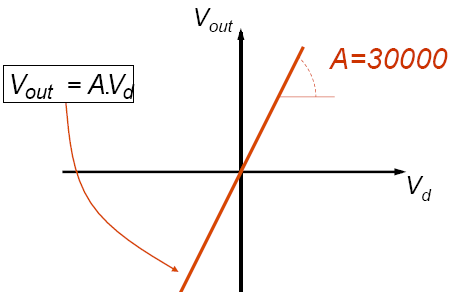
\includegraphics[scale=0.25]{img/image42}
\captionof{figure}{Caractéristique AOP}
\end{wrapfigure}
\subsubsection{Caractéristiques de transfert}

Un AOP possède plusieurs caractéristiques, mais nous nous intéressons ici à la \textit{caractéristique de transfert} c'est à dire le rapport entre la tension d'entrée $V_d$ et la tension de sortir $V_{out}$. Cette relation est déjà connue comme la loi fondamentale de l'AOP, loi qui se traduit par une droite de pente $A$.

\subsubsection{Caractéristique : zone linéaire}
\begin{wrapfigure}[8]{l}{3cm}
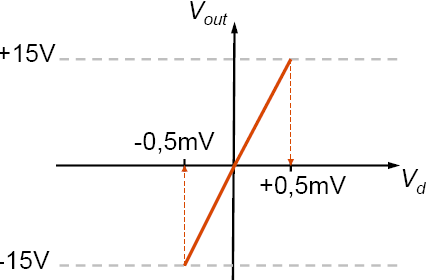
\includegraphics[scale=0.25]{img/image43}
\captionof{figure}{Zone linéaire}
\end{wrapfigure}
Il ne faut pas oublier de tenir compte d'un phénomène supplémentaire, à savoir :
\begin{equation}
-V_{al} \leq V_{out} \leq +V_{al}
\end{equation}
Ces limites se traduisent pas des horizontales dans le plan de la caractéristique. Seule la zone entre ces horizontales est accessible : il s'agit de la \textbf{zone linéaire}.\\
Les limites de cette zone sont simple à calculer, il s'agit des points de sortie pour lesquels $V_{d} = +V_{al}/A$ et $-V_{al}/A$. La grande valeur de $A$ a pour conséquence que la zone linéaire est très étroite sur l'axe horizontal.

\subsubsection{Caractéristique : saturation}
\begin{wrapfigure}[8]{r}{3cm}
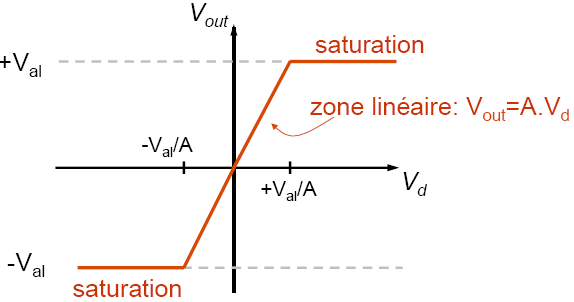
\includegraphics[scale=0.25]{img/image44}
\captionof{figure}{Saturation}
\end{wrapfigure}
Si la tension d'entrée est au-dessus de $+V_{al}/A$, la tension de sortie est \textit{limitée} à la valeur $+V_{al}$ : l'AOP ne peut aller plus haut que sa propre tension d'alimentation positive (et pareil pour la tension négative). Dans ces deux cas, lorsque l'on sort de la zone linéaire on dit que l'AOP \textbf{sature}.\\
\textbf{Attention !} Dans les zones de saturations, la loi fondamentale n'est plus vérifiée : il n'y a plus d'amplification.




\subsubsection{Principe du zéro virtuel}
Il s'agit d'une propriété générale de tous les AOP, propriété directement liée à la caractéristique de ce dernier. Cette propriété fondamentale permet de faire gagner beaucoup de temps et s'énonce :\\

\prop{\textsc{Principe du zéro virtuel :} Tant qu'un amplificateur opérationnel \textbf{ne sature pas}, sa tension différentielle d'entrée est virtuellement nulle.}\ \\

Il est important de ne considérer cette théorique seulement si l'AOP est en zone linéaire (\textbf{erreur classique!}). Une tension différentielle virtuellement nulle signifie que $V_d$ est tellement faible que l'on peut la négliger devant les autres tensions (souvent, $V_d \ll 1\ mV$). Négliger $V_d$ signifie l'approximation :
\begin{equation}
V_d = 0\ V
\end{equation}
C'est cette approximation que l'on appelle \textit{zéro virtuel}.\footnote{Zéro car $V_d$ est nulle, virtuel pour rappeler l'approximation.}


\subsubsection{Principe du zéro virtuel : remarques}
Quelques remarques sont à prendre en compte :
\begin{enumerate}
\item Compte tenu de la définition de $V_d$, le zéro virtuel revient encore à faire l'approximation :
\begin{equation}
V^+ = V^-
\end{equation}
\item La grande valeur de $A$ justifie ce principe. En effet, dans la zone linéaire $V_d$ est négligeable ce qui est évident au moment de tracer la caractéristique de transfert.
\item Le principe ne garantit \textbf{pas} que l'AOP est dans la zone linéaire.
\item Si l'on suit le principe, la tension d'entrée est nulle, or c'est elle que l'on veut amplifier... Problem ? No ! Le zéro virtuel fait \textbf{simultanément} deux approximations :
\begin{enumerate}
\item $V_d = 0\ V$
\item $A = \infty$
\end{enumerate}
La loi fondamentale devient une "forme indéterminée" et la valeur n'est pas forcément nulle; pas de contradictions.
\item Si l'on fait une des deux approximation du point précédent sans faire l'autre, on est foutu.
\end{enumerate}

\begin{wrapfigure}[9]{r}{3cm}
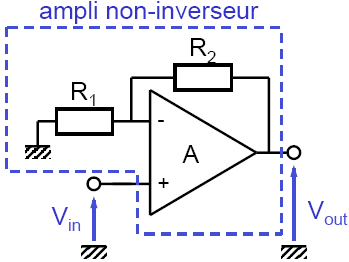
\includegraphics[scale=0.45]{img/image45}
\captionof{figure}{Schéma non-inverseur}
\end{wrapfigure}
\section{Deux montages amplificateurs}
\subsection{Ampli non-inverseur}
Un montage amplificateur inverseur est un ampli-op auquel on a ajouté deux résistances $R_1$ et $R_2$ dans le but de "contrôler" le gain. 

\subsubsection{Montage >< composant}
Il est fondamental de faire la différence entre "deux" niveau du schéma : l'AOP qui est le composant et le montage construit sur base de cet AOP. C'est l'ensemble complet que l'on appelle \textit{amplificateur non-inverseur}. Son signal d'entrée est $V_{in}$, son signal de sortie $V_{out}$. Ces deux tensions sont référencées à la masse, elle sont donc \textbf{non-}différentielles.\\

Sur la figure du schéma non-inverseur, la résistance $R_2$ placée entre la sortie de l'AOP et son entrée inverseuse : elle est en \textbf{rétroaction}. 


\subsubsection{Calcul du gain $A_{\text{non\_inv}}$}
Nous allons chercher à calculer le \textit{gain du montage} défini\footnote{$A_{\text{non\_inv}}$ est le gain "à vide", on suppose qu'aucune charge n'est connectée à la sortie du montage.} :
\begin{equation}
A_{\text{non\_inv}} = \frac{V_{out}}{V_{in}}
\end{equation}
Pour calculer ce gain, il faut choisir le modèle d'AOP que l'on utilise dans les calculs. Faisons les hypothèses suivantes et démontrons une expression du gain :
\begin{itemize}
\item Le gain $A$ est fini (élevé, mais pas infini).
\item Son impédance d'entrée $Z_d$ est infinie.
\item Son impédance de sortie est nulle.
\end{itemize}
\begin{proof}
\ \\
Considérons les deux relations fondamentales de départ, ré-écrite sous une seule identité :
\begin{equation}
\left\{\begin{array}{ll}
V_{out} & = A.V_d\\
V_d & = V^+ - V^-
\end{array}\right.\ \ \ \ \ \ \ \Rightarrow\ \ \ \ V_{out} = A.(V^+ - V^-)
\end{equation}
Essayons d'éliminer $V^+$ et $V^-$ au profit de $V_{in}$ et $V_{out}$ qui sont les variables à garder en finale. Comme $V_{in}$ est directement appliquée à l'entrée "+", on peut écrire :
\begin{equation}
V^+ = V_{in}
\end{equation}
On peut calculer $V^-$ par la méthodes des courants de branche, mais les propriétés de l'AOP permettent d'aller un peu plus vite. Posons qu'il existe un courant $I$ traversant $R_2$. Lorsque ce courant quitte $R_2$, il ne peut rentrer dans l'AOP car l'impédance de celui-ci est infinie : $I$ doit donc passer en totalité dans la résistance $R_1$.

\begin{center}
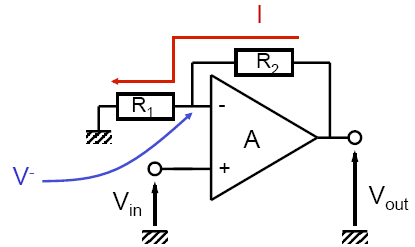
\includegraphics[scale=0.45]{img/image46}
\captionof{figure}{Schéma pour le calcul de $V^-$}
\end{center}

 En appliquant la loi d'Ohm sur chacune des résistances, on peut éliminer $I$ pour obtenir notre troisième équation : 
\begin{equation}
\left\{\begin{array}{ll}
V^- & = R_1I\\
V_{out} - V^- & = R_2I\\
\rightarrow V_{out} & = (R_1+R_2)I
\end{array}\right.\ \ \ \ \ \ \ \Rightarrow\ \ \ \ V^- = \dfrac{R_1}{R_1+R_2}V_{out}
\end{equation}
Notons que ce résultat aurait pu être immédiat par application du diviseur résistif, sous l'hypothèse que $Z_d = \infty$.\\ En combinant nos trois équations obtenues, on trouve l'équation
\begin{equation}
V_{out} = A\left(V_{in} - \dfrac{R_1}{R_1 + R_2}V_{out}\right)
\end{equation}
qu'il suffit de réarranger pour obtenir le gain recherché :
\begin{equation}
A_{\text{non\_inv}} = \frac{V_{out}}{V_{in}} = \frac{A(R_1+R_2)}{AR_1+R_1+R_2}
\end{equation}
La valeur élevée de $A$ permet de négliger $R_1$ et $R_2$ par rapport à $AR_1$. On trouve finalement le gain de notre AOP :\\

\prop{$A_{\text{non\_inv}} \approx 1 + \frac{R_2}{R_1}$}
\end{proof}

\subsubsection{Amplificateur non-inverseur : remarques}
Si ce montage est dit "non-inverseur", c'est parce que son gain est positif. On remarque également que le gain de l'AOP ($A$) n'est pas dans l'expression de $A_{\text{non\_inv}} \rightarrow$ le gain du montage ne dépend pas du gain de l'AOP mais uniquement des valeurs des deux résistances. Les deux sous-sections précédentes sont consacrées à deux de ses propriétés.

\subsubsection{Montage non-inverseur à gain variable}
Régler le gain peut être fondamental, comme par exemple pour régler le volume de votre amplificateur audio. Pour se faire, il suffit de remplacer une des deux résistances (le plus souvent $R_2$, car étant au numérateur elle donne une variation linéaire du gain) par un \textit{potentiomètre}. Pour rappel :\\

\prop{Un potentiomètre est une résistance variable dont l'utilisateur règle la valeur via un curseur mécanique.}\ \\



%\subsubsection{Impédance d'entrée}

\subsection{Ampli inverseur}
\begin{wrapfigure}[7]{r}{3cm}
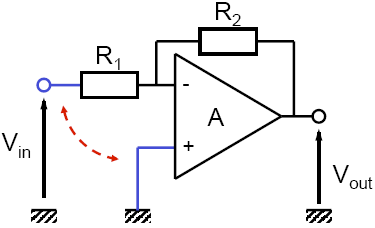
\includegraphics[scale=0.35]{img/image47}
\captionof{figure}{Schéma inverseur}
\end{wrapfigure}
Ce montage à base d'un AOP est quasi-identique au non-inverseur à une exception près : le rôle de la masse et de l'entrée $V_{in}$ ont été permuté :
\begin{itemize}
\item $V_{in}$ est maintenant connectée à $R_1$
\item L'entrée "+" est maintenant mise à la masse
\end{itemize}
Notons cependant que $R_2$ est toujours montée en rétroaction (entre l'entrée et la sortie) et que $R_1$ et $R_2$ forment toujours un diviseur résistif (un peu particulier, car aucune des extrémités n'est à la masse).

\subsubsection{Calcul du gain $A_{inv}$}
En utilisant la méthode de calcul classique du point précédent (même hypothèses et démarches de calcul), on trouve que le gain à vide vaut :

\prop{\begin{equation}
A_{inv} \approx -\frac{R_2}{R_1}
\end{equation}}

\begin{proof}\ \\
Afin de calculer la réponse en fréquence de ce circuit, il faut tout d'abord modéliser
    l'amplificateur opérationnel par un élément d'impédance d'entrée infinie, d'impédance
    de sortie nulle et de tension de sortie :
    
        \begin{equation}
        V_{\text{out}}=A(V^+ - V^-)
        \end{equation}
    où A est le gain propre à l'amplificateur, très élevé, mais fini. Le gain à vide du montage
    étant:
        \begin{equation}
        G = \frac{V_{\text{out}}}{V_{\text{in}}}
        \end{equation}
    
    Deux autres équations sont encore nécessaires pour arriver à  calculer le gain de notre
    amplificateur inverseur. Premièrement, nous savons que la borne positive est directement
    connectée à la masse. Deuxièmement, en utilisant la loi des mailles et en supposant qu'un
    même courant $I$ circule dans les résistances $R_1$ et $R_2$ (l'amplificateur possédant
    une impédance d'entrée infinie). Nous obtenons dès lors :

        \begin{equation}
            \left\{\begin{array}{l}
             V^+=0  \\
             V_{\text{in}}+R_1 I + R_2 I = V_{\text{out}}
            \end{array}\right.
        \end{equation}
    Sachant que $V^-=V_{\text{in}}+R_1 I$, nous obtenons l'équation :
        \begin{equation}
        V^-=V_{\text{in}}+R_1\frac{V_{\text{out}}-V_{\text{in}}}{R_1+R_2}
        \end{equation}

    Nous pouvons désormais exprimer $V_{\text{out}}$ en fonction de $V_{\text{in}}$ :
        \begin{equation}
        V_{\text{out}}=-A\left( \dfrac{V_{\text{in}}(R_1+R_2)+R_1 V_{\text{out}}-R_1 V_{\text{in}}}{R_1+R_2}\right) = -\dfrac{R_2 V_{\text{in}}+R_1 V_{\text{out}}}{R_1+R_2}
        \end{equation}
    Ou encore, après ré-arrangement :
        \begin{equation}
        (A R_1 + R_1 + R_2) V_{\text{out}} = -A R_2 V_{\text{in}}
        \end{equation}
    En supposant que $A R_1$ est beaucoup plus grand que $R_1 + R_2$, nous pouvons exprimer le 
    gain de notre amplificateur inverseur :
     \begin{equation}
     G =-\frac{A R_2}{A R_1 + R_1 + R_2} \approx -\frac{R_2}{R_1}
     \label{eq:gain}
     \end{equation}
\end{proof}

\subsubsection{Amplificateur inverseur : remarques}
Si ce montage est dit "inverseur" c'est parce que son gain est négatif. Comme pour le non-inverseur, le gain $A$ à également disparu de l'expression de $A_{inv}$. Comme avant, le gain peut être rendu variable à l'aide d'un potentiomètre si ce n'est qu'ici le gain minimal est nul !

\newpage
\subsubsection{Impédance d'entrée : calcul}
\begin{wrapfigure}[8]{l}{3.5cm}
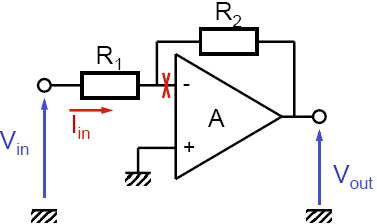
\includegraphics[scale=0.35]{img/image48}
\captionof{figure}{Calcul de $Z$}
\end{wrapfigure}
Calculons l'impédance d'entrée du montage inverseur. 
\begin{equation}
Z_{in} = \frac{V_{in}}{Z_{in}}\left|_{I_{out} = 0}\right.
\end{equation}
Le courant $I_{in}$ circulant n'est autre que celui circulant dans $R_1$, mais également celui circulant dans $R_2$ (l'impédance de l'AOP étant infinie). On peut donc écrire que ce courant vaut (loi d'Ohm sur l'ensemble des deux résistances) :
\begin{equation}
I_{in} = \frac{V_{in} - V_{out}}{R_1+R_2}
\end{equation}
Par définition de l'AOP inverseur, $V_{out}$ vaut :
\begin{equation}
V_{out} = A_{inv}.V_{in} = -\frac{R_2}{R_1}V_{in}
\end{equation}
En combinant les deux équations fraichement trouvées, on trouvé la valeur de $I_{in}$
\begin{equation}
I_{in} = \frac{V_{in} + \frac{R_2}{R_1}V_{in}}{R_1+R_2} = \frac{V_{in}}{R_1}
\end{equation}
L'impédance d'entrée vaut dès lors :
\begin{equation}
Z_{in} = R_1
\end{equation}
Il ne faut surtout pas conclure que l'impédance d'entrée du \textbf{montage} c'est "l'impédance qui se trouve à l'entrée du montage", résultat totalement faux dans le cas général ! Il faut dire que $Z_{in}$ à la même valeur que $R_1$ (sans l'être).\\

Cette impédance d'entrée est donc relativement faible (on pouvait s'attendre à ce qu'elle soit très élevée au vu de l'analyse du non-inverseur) doit être vue comme un inconvénient du montage inverseur.

\subsubsection{Méthode de calcul classique}
La méthode de résolution que nous avons utilisé tout au long du chapitre permet de résoudre tout circuit AOP avec rétroaction. Elle permet de calculer le gain à vide mais aussi de calculer l'impédance d'entrée sous hypothèses que l'impédance d'entrée d'un AOP soit aussi hight que Buzz.

\subsection{Calcul rapide par le principe du zéro virtuel}
Le principe du zéro virtuel énoncé précédemment permet d'effectuer un calcul beaucoup plus rapide qu'avec la méthode classique\footnote{Cela implique qu'on suppose $A = \infty$ dès le départ.}.

\newpage
\subsubsection{Calcul du gain de l'AOP non-inverseur}
\begin{wrapfigure}[8]{r}{3.5cm}
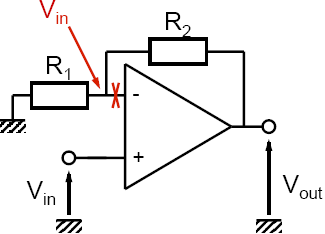
\includegraphics[scale=0.35]{img/image49}
\captionof{figure}{AOP N-I}
\end{wrapfigure}
Commençons par poser nos différentes hypothèses sur l'AOP : impédance différentielle $Z_d$ infinie, impédance de sortie null et l'on a un zéro virtuel (gain de l'AOP infini et $V_d = 0$).\\
La "loi" n'est \textbf{plus} à utiliser ici ! De plus utiliser $A$ peut poser problème (comme supposé infini). A la place, ayant un zéro virtuel, on peut écrire $V^+ = V^- \rightarrow$ cette équation nous servira de "première équation". \\
Notre système d'équation est ainsi :
\begin{equation}
\left\{\begin{array}{ll}
V^+ &= V^-\\
V^+ &= V_{in}\\
V^- &= \frac{R_1}{R_1+R_2}V_{out}
\end{array}\right.
\end{equation}
En vertu de la première équation, on peut immédiatement égaler les deux équations de droite et trouver directement le gain du montage
\begin{equation}
A_{non_inv} = \frac{V_{out}}{V_{in}} = 1+\frac{R_2}{R_1}
\end{equation}
Ce qui est bien le même que celui obtenu avec la méthode classique.\\

C'est bien beau, mais on peut encore faire mieux en raisonnant "directement sur le schéma" tout en limitant les développement mathématiques :
\begin{enumerate}
\item Dans l'hypothèse du zéro virtuel, $V^- = V^+$
\item Or $V^+$ vaut $V_{in}$, ceux-ci étant en connexion directe
\item Donc, $V^-$ vaut $V_{in}$
\item Par ailleurs, $R_1$ et $R_2$ forment un diviseur résistif (car aucun courant ne passe dans l'AOP ($Z_d = \infty$)
\item Pour ce diviseur résistif, on peut donc écrire
\begin{equation}
V_{in} = \frac{R_1}{R_1+R_2}V_{out}
\end{equation}
Dont on déduit directement le gain
\begin{equation}
A_{non_inv} = \frac{V_{out}}{V_{in}} = 1+\frac{R_2}{R_1}
\end{equation}
\end{enumerate}

En terme de rapidité, on ne peut faire mieux ! Mais : il faut bien maîtriser les concepts de la théorie et les appliquer au bon moment! 

\subsubsection{Calcul du gain de l'AOP inverseur}
\begin{wrapfigure}[8]{r}{3.5cm}
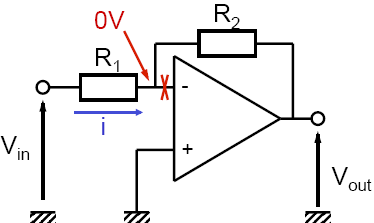
\includegraphics[scale=0.35]{img/image50}
\captionof{figure}{AOP I.}
\end{wrapfigure}
Travaillons directement sur le schéma :
\begin{enumerate}
\item Dans l'hypothèse du zéro virtuel, $V^- = V^+$
\item Or $V^+$ vaut $0V$ : connexion directe à la masse
\item Donc $V^-$ vaut 0 $V$ (on parle de "masse virtuelle")
\item Par ailleurs, $R_1$ et $R_2$ forment un diviseur résistif (car aucun courant ne passe dans l'AOP ($Z_d = \infty$) (non "classique" car on a 0V au milieu des deux résistances)(j'aime les parenthèses)
\item Le courant dans $R_1$ est facile à trouver :
\begin{equation}
I = V_{in}/R_1
\end{equation}
En effet, comme l'extrémité droite de $R_1$ est (virtuellement à à la masse, la ddp sur $R_1$ vaut bien $V_{in}-0V = V_{in}$.
\item Comme ce même courant passe dans $R_2$, on peut écrire : $0V-V_{out} = R_2I$. On trouve finalement
\begin{equation}
V_{out} = -R_2I = -R_2\left(\frac{V_{in}}{R_1}\right)
\end{equation}
ou encore
\begin{equation}
A_{inv} = \frac{V_{out}}{V_{in}} = - \frac{R_2}{R_1}
\end{equation}
\end{enumerate}


\subsection{Analyse de la rétroaction}
Les deux montages vu précédemment comportent tous deux une résistance $R_2$ en rétroaction. Clarifier le fonctionnement de cette rétroaction peut répondre à un certains nombres de questions : pourquoi amplifier $V_d$ et pas $V_{in}$, que justifie l'hypothèse du zéro virtuel ?

\subsubsection{Analyse de la rétroaction : principe}
Au cours de notre raisonnement, nous adopterons deux règles :
\begin{enumerate}
\item Raisonner strictement en termes de "cause" et d'"effet"
\item L'AOP régit avec un certain délai : raisonnons plus vite que lui ; supposons que la tension de sortie de l'AOP ne peut subir de discontinuité (échelon)
\end{enumerate}


\subsection{Compléments sur la rétroaction}




\section{Montages à ampli-op}
\section{Ampli-op : propriétés avancées}


\part{Électronique numérique}
\setcounter{chapter}{9}
\chapter{L'électronique numérique, c'est quoi ?}
\end{document}


